% THIS IS SIGPROC-SP.TEX - VERSION 3.1
% WORKS WITH V3.2SP OF ACM_PROC_ARTICLE-SP.CLS
% APRIL 2009
%
% ----------------------------------------------------------------------------------------------------------------
% This .tex file (and associated .cls V3.2SP) *DOES NOT* produce:
%       1) The Permission Statement
%       2) The Conference (location) Info information
%       3) The Copyright Line with ACM data
%       4) Page numbering
% ---------------------------------------------------------------------------------------------------------------
% For tracking purposes - this is V3.1SP - APRIL 2009

\documentclass{acm_proc_article-sp}
\usepackage{graphicx}
\usepackage{hyperref}
\usepackage{amsmath}
\usepackage{float}
\usepackage{caption}

\makeatletter
\def\@copyrightspace{\relax}
\makeatother

\begin{document}
%work on this title
\title{Clipit: An Intelligent Clipboard Manager for Programmers}
\subtitle{Design, Development, and Evaluation of Three Feature Sets \thanks{This report is Group G's April 7 Deliverable for CSC 510 taught by Dr. T. Menzies in the Spring of 2016 at North Carolina State University.}}

\numberofauthors{4} 
\author{
\alignauthor
Brian Clee\\
       \email{bpclee@ncsu.edu}
\alignauthor
Effat Farhana\\
       \email{efarhan@ncsu.edu}
\and % go to new row
\alignauthor
Arjun Madan\\
       \email{amadan2@ncsu.edu}
\alignauthor
Ran Tan\\
       \email{rtan2@ncsu.edu}
}

\date{7 April 2016}
\maketitle

%maybe consider everytime we mention clipit we italicize it? Like so: \textit{Clipit}
\begin{abstract}
The copy and paste command is the basic mechanism for duplicating part of a document in the same or another document. It can be performed through various means (e.g. using the keyboard, mouse-based direct manipulation, or menus). In this paper, we aim to facilitate the programmer's need to enhance their productivity while copying and pasting code blocks. Our project targeted the open-source Atom text editor and designed/developed three unique feature sets on an existing clipboard manager package. We then conducted experiments comparing among our newly added features and documented the best feature based on our empirical observations and user feedback. 

\end{abstract}

%see http://www.acm.org/sigs/publications/sigguide-v2.2sp section 2.3.2
% A category with the (minimum) three required fields
\category{D.2.2}{Software Engineering}{Design Tools and Techniques}[Modules and interfaces, programmer workbench, user interfaces]
%A category including the fourth, optional field follows...
\category{D.2.3}{Software Engineering}{Coding Tools and Techniques}[Program Editors]

% see http://www.acm.org/sigs/publications/sigguide-v2.2sp section 2.3.3
\terms{Human Factors, Management, Performance, Theory}

\keywords{Code duplication, copy and pasting, program editors, programmer habits, programmer productivity}

\section{Introduction}\label{sec:intro}

In the field of computer programming, developers frequently make use of the copy and paste operation for numerous reasons. For one, it is essential in the practice of relocating, regrouping, or reorganizing code from one place to another. Along these lines, programmers also use the command in the act of reordering parts of their code, rather than rewriting them. Finally, perhaps the most common use of the copy and paste command is when a programmer copies a block of code, either from inside sources within their existing code base or outside it, to use as a structural template~\cite{ooplCP}.

To make the process of copying and pasting more efficient for programmers we outlined in our February 1 report~\cite{janReport} the need for an effective clipboard manager designed specifically for programmers.

After researching possible target platforms to develop our clipboard manager variation on, we eventually decided to create plugins for Atom~\cite{Atom}, an open source text editor. In Atom, plugins are referred to as packages, and due to the open-source nature of the platform all packages for the editor are open-sourced themselves. 

We chose the Atom platform for a number of reasons, for starters atom is an open-source platform. This might seem like a trivial benefit, but this allows us to completely customize any aspect of its functionality. 

Another reason why we chose Atom was the built in package support included in the editor. Located inside the main editor settings panel, Atom provides helpful development functions like package search, install/remove, and disable/enable. Furthermore, at its core Atom provides a structured way to develop and test packages with built in developer tools.

Finally, a core requirement for our team was multi-platform support. As two of our group members were Mac users and two of our group members were Windows users, it was necessary to choose an editor which provided multi-platform support. In Atom's case, the way in which packages are developed allows developers to put in relatively little extra effort to get packages working across Windows, Mac, and Linux systems. 

Once we had chosen Atom as our target platform and development environment, we then researched through the myriad of existing packages already available for Atom. Most of these packages were unrelated to our project, but we did end up finding an Atom package called clipboard-history~\cite{Atom_C_History} which provided basic clipboard history functionalities. For us this was a perfect base to start our own development from and it greatly reduced our start up programming time as we were able to avoid starting completely from scratch. After altering the source package code of clipboard-history into our own base version we renamed this package Clipit and will refer to it as such for the rest of this report.

After we had selected our development platform, and the base project we were going to work off of, we then returned to our February 1 report~\cite{janReport} to finalize the design of our three features. Focusing on the average programmer's habit of copying and pasting our first feature, Clipit-order, was designed to provide contextual ordering of copy-paste items. More specifically, this means sorting code blocks/items by most frequently copied/pasted, sorting by timestamp, and finally sorting based on the source file items were copied from.

The second feature we designed is called Clipit-panel, and as the name suggests provides a user interactive display panel to show copied items statically. This is critically different from the base version which only shows the clipboard history dynamically through a command press. By showing items statically at all times to the users it allows programmers to constantly browse the list of copied items, and paste directly from the panel.

The third and final feature we designed is called Clipit-cmd. This feature was made specifically with ``power-users'' in mind, as it provides complete keyboard command based interactions to quickly traverse the clipboard history. Essentially Clipit-cmd re-imagines the clipboard history as a stack, and gives users commands to traverse up and down the stack, to then paste from their current stack position.
 
Throughout the body of this report we will discuss our overall project synopsis, including more detailed discussions of each of the features in section~\ref{sec:synopsis}. Our experimental design, methodology, and participant selection is discussed in section~\ref{sec:experiment}. Following this our results are laid out and explained in graphical format in section~\ref{sec:results}. Finally conclusions and comparisons are made on our results, we declare our best feature, and future work is outlined in section~\ref{sec:discussion}.

\section{Synopsis}\label{sec:synopsis}

In this section we talk about the work done previously in studying copying and pasting habits of users, the common problems people face, and our three features that greatly improve copying and pasting, especially for programmers.

\subsection{Previous Work}\label{sec:previous}

Previous research~\cite{devWorkHabits} showed that software developers spend a considerable amount of time copying and pasting while programming, and while a good default system is in place, there is scope for a lot of improvement. A study conducted by IBM on the work flow behavior of programmers has shown that programmers copy and paste on average 16 times per hour while developing software~\cite{ooplCP}. We found previous solutions did exist~\cite{overlapWindow}~\cite{cpHabits} to improve copy and paste functionality, but were old, and not actively being developed anymore. They also lacked some basic features we felt were essential when focusing on programmers. 

A lot of our initial research~\cite{janReport} was focused on improving these tools, and coming up with a list of features we thought would help improve a programmers productivity by not only making copying and pasting faster, but also by reducing the errors people made while carrying out these operations~\cite{maintenenceStudy}.

Previous research~\cite{cpHabits} also showed that programmers spent a considerable portion of their time on switching windows in order to select the text they wanted to copy and then pasting it at the required destination. We proposed a multi-item clipboard, that allowed people to copy multiple items from different windows into a clipboard history, and then cycle through them in order to paste the correct one, thereby reducing the number of window switches required per paste. We consider this multi-item clipboard as the base version for our solution, and propose three separate features that add on to this.

\subsection{Features}\label{sec:features}

For our purposes of streamlining development, and not reinventing the wheel, the open-source Atom package clipboard-history~\cite{Atom_C_History} was used as our starting point of development, and renamed to Clipit. Clipit enables a multi-item clipboard in the form of a visual clipboard history which can be accessed through a keyboard command, as users copy items this history is populated. We developed three unique features, detailed in section~\ref{sec:intro}, that added value to this package and sought to achieve the goals laid out in our initial research~\cite{janReport}.

\subsubsection{Clipit-cmd}\label{sec:features_cmd}

Most programmers are familiar with using keyboard shortcuts, without receiving any visual response, and Clipit-cmd focuses entirely on this. Clipit-cmd works by adding content a user copies as separate items in a list. The number of items in the list is tracked, and initially the cursor is on the most recent item in the stack. Programmers can use keyboard shortcuts to cycle through this list and when they try pasting an item, the item being currently pointed to by the cursor is returned. This would allow a user to have multiple items stored in the list, and instead of having to switch windows and re-find the text to be copied, they just need to cycle through the list and paste the required item. 

\subsubsection{Clipit-order}\label{sec:features_order}

One of the drawbacks of Clipit-cmd is that when the list grows very large, programmers often lose track of where items are located in the list. Clipit-order aims to remedy this problem by having the list being shown as a pop-up with a section of the chunk of code, along with a preview that shows more, when selected. Clipit-order also allows users to contextually sort the items based on the frequency of copies, time an item was last copied or pasted, or group items by the source file from they were copied from. This gives users more flexibility in terms of how they want to have their copies organized. Users also had the option to enter a search query that would filter the list and show only the items with the words in the search query. Users can also clear all items from the panel, to keep it more manageable. Clipit-order also supports data persistence, a feature that allows items to remain on Clipit-order's clipboard, even after Atom has been restarted. This is especially useful when a user is working on a project over days.

\subsubsection{Clipit-panel}\label{sec:features_panel}

Clipit-panel is a persistent panel that exists on the right edge of the screen. When items are copied, they are added to the clipboard. In order to paste an item from the clipboard, the user just has to click on the item, and the content is pasted at the location of the cursor. The top item on the list is expanded, and only snapshots of the subsequent items in the list are shown, so as to maximize the amount of space available. In addition to this, a search bar like the one in Clipit-order is present here to make it easier for the user to find what they're looking for. Users also have the option to clear their panel, where all items copied are removed from the panel. This helps keep unnecessary items of the panel and keep it manageable.

\section{Experiment}\label{sec:experiment}

\subsection{Task Methodology}\label{sec:task}
In order to test the three features of Clipit (Clipt-cmd, Clipit-panel, and Clipit-order), and see how  effective they are in practice, we designed an experiment that tested the participants on copying and pasting blocks of code in a real project. The experiment had participants build the base version of clipboard-history, the open source clipboard manager for Atom we based our project on. Parts of the code were removed and placed across four source files from which the participants had to copy the code and paste it in the correct place, in order to eventually get a working version of clipboard-history. Comments were left, and detailed instructions were provided in the form of tasks~\cite{Tasks}, so that the participants had enough information to successfully complete all the assigned copy and pastes to rebuild the project.

The tasks were designed in a way to focus on the different areas of each Clipit feature, with different tasks meant to favor different features. The areas we focused on with the tasks were:

i. Copying the source from multiple windows, inside the editor.\\
ii. Copying the source from multiple windows, inside and outside the editor.\\
iii. Copying the source multiple times from the same file.\\
iv. Pasting across multiple files.\\
v. Pasting multiple times to the same file.

In order to get quantitative results from the experiment, we logged each copy, and paste, along with the content and time it occurred. This allowed us to not only capture the time it took each participant to complete all the tasks, but also calculate the time taken for each task which allowed us to analyze the results in greater detail, as shown in section~\ref{sec:results} and discussed in section~\ref{sec:discussion}.

\subsection{Participants}\label{sec:participants}

The participants were selected based on their knowledge of programming, and familiarity with copying and pasting. They were asked to fill out a pre-survey, following which 8 respondents were chosen to participate in the experiment. The eight participants were all Computer Science graduate students at North Carolina State University, with half of them in the process of completing their Master's degree, and the other half in the process of obtaining a Ph.D. 

All the participants had more than a year of programming experience, and 37.5\% of them had more than 3 years of experience. 62.5\% of the participants also had more than 3 months of industry work experience, and everyone was at least familiar with concept such as requirements engineering, and creative coding. 

Most importantly, Figure \ref{fig:Frequency} shows us that 37.5\% of the participants reported that they frequently use copying and pasting while programming, with the remaining 62.5\% using these techniques sometimes.

\begin{figure}[h]
\centering
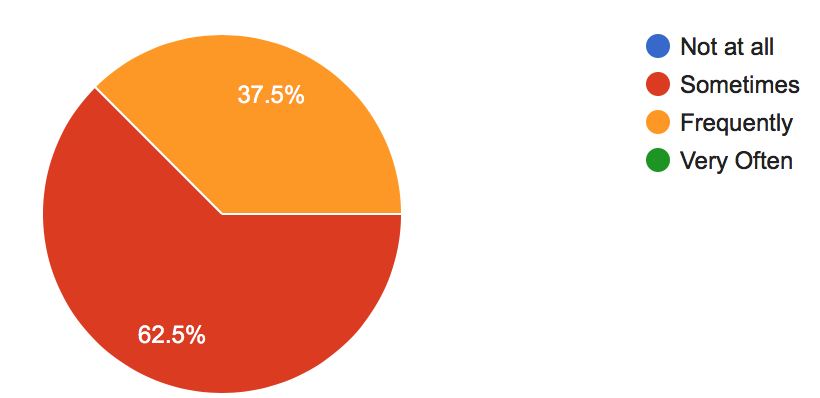
\includegraphics[width=6cm]{frequency}
\caption{Copy and paste frequency among programmers}
\label{fig:Frequency}
\end{figure} 

\section{Results}\label{sec:results}

After the experiments were conducted, the data collected was analyzed in order to check for the presence of any interesting patterns.

To begin with, Figure \ref{fig:group} lists the per-task completion time for each feature.

\begin{figure}[h]
  \begin{minipage}{0.50\textwidth}
    \centering
    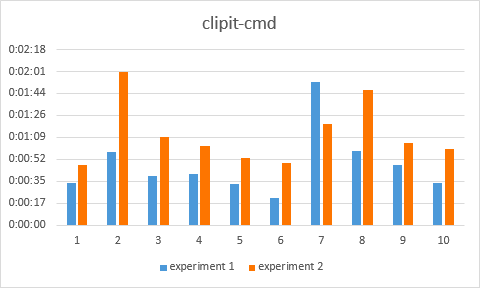
\includegraphics[width=.45\textwidth]{cmd_tasks}\quad
    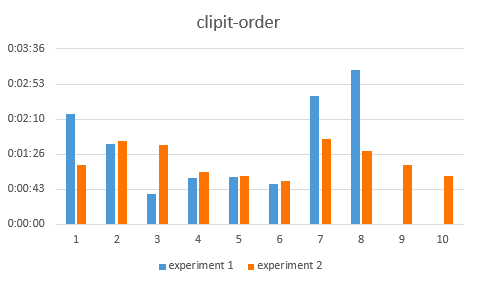
\includegraphics[width=.45\textwidth]{order_tasks}\\
    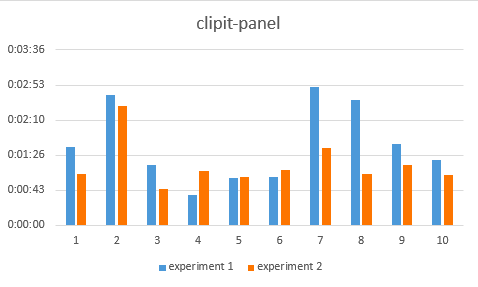
\includegraphics[width=.45\textwidth]{panel_tasks}\quad
    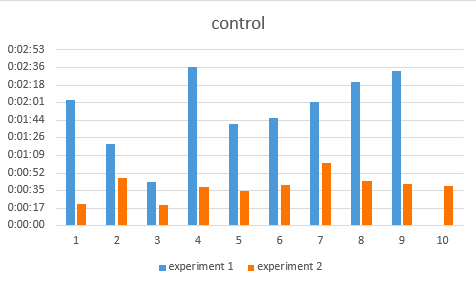
\includegraphics[width=.45\textwidth]{control_tasks}
    \caption{Per task completion time for each feature}
    \label{fig:group}
  \end{minipage}
\end{figure}

The bar graphs in \ref{fig:group} also show that Task 2 and Task 8 took the most time for participants to accomplish. The task descriptions~\cite{Tasks} for the tasks clearly indicate that Task 7 and Task 8 simply require more copy and paste operations than the other tasks, which explains the per-task completion time peeks at Task 8. However, Task 2 was not as complex as task 8, and took roughly the same amount of time. We attribute this to the fact that the participants were not familiar with the features being tested, and took a few tasks to get used to using them, indicating there is a learning curve to using these features. This assumption is strengthened by analyzing the time taken to complete Task 2 with the control group, which was at least 40\% less than that taken by the other groups.

To further understand the experiment results and evaluate each feature, comparisons are made between features. Figure \ref{fig:avg-time} shows us the average completion time for each feature. We see that Clipit-cmd performed better than control, while Clipit-order and Clipit-panel didn't. This is a strong empirical vote for Clipit-cmd to be the best feature, and we will discuss this further in section~\ref{sec:bestfeature}.

\begin{figure}[h]
\centering
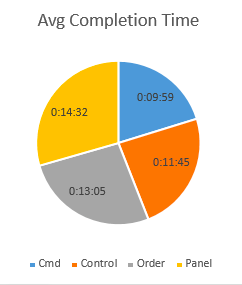
\includegraphics[width=6cm]{avg_time}
\caption{Average completion time for each feature}
\label{fig:avg-time}
\end{figure}

To get a closer look at the average completion time for each tasks, Figure \ref{fig:per-avg-time} compares all four features on each task. The bar graph shows us that participants using Clipit-cmd took the least time to complete most of the tasks. However, we also seee that that control performed better at Task 3 and Task 10, which was quite unexpected. As mentioned previously in section~\ref{sec:participants}, for the case of Task 3, we believe this could be due to the fact that participants had to learn how to use the feature, and this is the reason for them taking longer to accomplish the task.


\begin{figure}[h]
\centering
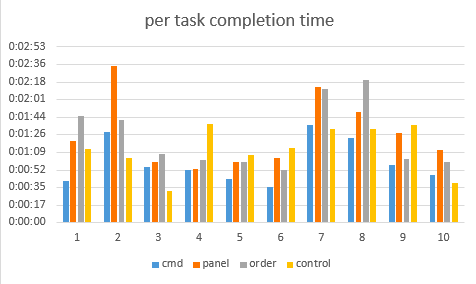
\includegraphics[width=6cm]{per_task_avg}
\caption{Per task average completion time for each feature}
\label{fig:per-avg-time}
\end{figure}


\section{Discussion}\label{sec:discussion}

After conducting our experiments and gathering our results we were able to come up with numerous conclusions. For one, it became obvious by the end of our testing cycle that there were a myriad of changes that could be made to each of our feature sets. As the designers and developers we had a narrow view entering testing that each of the features we had developed were mostly complete, albeit with a few known issues and disadvantages here and there; however, upon completing our testing it became clear that there each of our features had many more flaws than we initially accounted for. Yet it should also be noted that the criticism we gathered was for the most part constructive, and on the whole each of our testers enjoyed using our features and had many good things to say about them. 

This section of the report focuses on the overarching takeaways we gained from our experiments, and discusses which of the features is empirically "the best", while also focusing on the strengths and weaknesses of each of our features. We will back up these claims with data taken directly from our experiments discussed in section~\ref{sec:results}, as well as from our pre and post surveys that were filled out by all study participants. Finally, we will discuss the future work that could be done with each of the features to address their individual criticisms and solve usage issues encountered by our study participants.

\subsection{Observations and Limitations}

When we initially designed our experiments we had a naive notion that through our experiments we would be able to reaffirm what we already understood about our features we had developed in terms of their advantages and disadvantages. Of course, after completing our experiments we quickly realized that each of these features had benefits we had not foreseen, as well as numerous drawbacks. Furthermore, each of our features had their own unique observations that weren't always shared across our project, and for that reason we will discuss each of them individually.

\subsubsection{Clipit-cmd}

To start, Clipit-cmd was perhaps the most demanding feature to use as it required learning how a clipboard history can function as a stack, and then further learning two commands for navigating through that stack. As well, there is a high overhead of effort when using this feature as it requires the user to constantly have a mental map of where they are located currently on the stack, as well as what the stack contains. Our experimental observations affirmed these findings, participants mentioned the lack of any visual component alerting them to their current location and stack contents as a desired addition. Participant's also frequently mixed up the two commands at first, confusing one for the other, or at some points simply not knowing if they were using the right keys at all. Furthermore during our post-surveys, participants who used Clipit-cmd rated it on average as the hardest to initially learn how to use; however, interestingly enough in a follow up question Clipit-cmd rated as one of the easiest to use on average, once the initial learning curve had been overcome.

On the whole all of these issues could be addressed with the addition of a visual component to this feature, as it would seamlessly remind users of their current location on the stack, the contents of the stack, and alert the users what their command entries are actually doing. By including a subtle visual component that isn't too distracting Clipit-cmd would have a lower cognitive load associated with its use, and users would be able to use it more effectively than they currently were during our experiments. As well, adding a visual component would reduce the initial learning curve and get users comfortable using the package quickly.

Additionally, with all of that being said, it should be noted that despite these learning issues, Clipit-cmd still had the fastest completion times for the experiment across all participants. This is further discussed in section~\ref{sec:bestfeature}.

\subsubsection{Clipit-order}

On the whole, Clipit-order was the most functionally and visually similar feature to our base version that our project started from. What differentiated Clipit-order from our base project was obviously the contextual ordering options that the feature provided, which allowed users to sort by time, source, and frequency. Unfortunately, embedding the use of these contextual ordering into our task design was quite difficult to do, as they naturally lend themselves to longer work sessions, and we were designed for shorter overall experiments, see section~\ref{sec:experiment}. 

Because of this, neither of our experiment participants fully explored this feature, and instead mainly used the package in it's default time sort. Nevertheless, we were still able to gather key observations on this feature's usage. 

For one, it seemed like an easy addition to this feature would be tweaking the sorting behavior such that when a user types the command to sort by a specific context, the clipboard history is immediately shown with that ordering. One participant was slow to perform their first few tasks because they thought they were hitting the wrong sort commands as the expected this functionality to already be implemented. This is an easy addition, and one that would speed up overall usage of this feature. 

As well, since this feature encourages filling up the clipboard history with lots of items, another participant noted that they wished their was a keyboard command to clear their clipboard history. As it works now, the user has to scroll to the bottom of the history to find the clear button, and if they didn't know that button existed by the time numerous items had been copied they wouldn't have ever been aware it was an option.

Overall, our observations and user feedback from post-surveys leads us to believe that in long term project development Clipit-order would perhaps be the best feature to use. This is mainly because the power of contextual ordering options really only exhibits itself when there are hundreds of copies made across numerous sources, otherwise the frequency and source sort options really don't factor into normal workflow whatsoever (as evidenced by their lack of use by our study participants).

Empirically speaking, Clipit-order was the second best feature in terms of the time it took participants to finish all tasks. 

\subsubsection{Clipit-panel}

Our observations of Clipit-panel were initially exactly what we had expected going into testing. Due to the severe nature of the formatting issue with this feature that auto extends the width of the panel to the width of the user's copy, it can be quite jarring to use this feature, and at certain times completely unusable. The study participants immediately picked up on the formatting issue and complained about it, but all the same they found ways to use the feature successfully even with the formatting issues. 

When looking at the total time to complete all of the tasks, Clipit-panel actually had the worst average completion time, being a full minute and a half slower than Clipit-order on average. This came as a suprise to us, as we hypothesized that the static nature of the panel would speed up usage over features like Clipit-order which essentially displayed the exact same information through more key-presses. Nevertheless this feature was empirically the slowest, and this is most likely due to the time participant's had to spend working around the formatting issues of the feature.

In the post-surveys for this feature both participants of course noted the formatting issues, but also went out of their ways to explain that on the whole they really liked the feature and if this bug would be addressed they would probably use the feature in their daily work flow. One participant summed up their thoughts nicely by saying "again, [Clipit-panel] worked as I expected, but there were a few bugs which prevented fluid work, like intrusive resizing of the window (horizontally), resizing of elements in the list (vertically), [and] inconsistency of whether a newly selected copy would paste with one clicks or two."

Clearly Clipit-panel shows promise, and could even potentially outperform Clipit-order in terms of task completion time if the formatting issues are addressed.

\subsection{Best Feature}\label{sec:bestfeature}

As discussed in the previous section, based on the results of our experiments Clipit-cmd is the best feature. This conclusion is reached through a couple of different methods. The most obvious one is based on our empirical results from our experiment discussed in section~\ref{sec:results} which show that the participants who used Clipit-cmd on average finished all of the tasks 3 minutes faster than any other feature (and roughly 2 minutes faster than the control group).

Additionally, even though in post surveys participants said that Clipit-cmd had a high learning curve at first, they later responded that once that had learned how to use the feature it was overall an easy to use package. Participants also stated that they "liked the simplicity and ability to control [the clipboard history] entirely through commands", and also stating that "the feature was straightforward to use". Furthermore, when participants were asked if they would be likely to use their feature in their everyday work flow, Clipit-cmd was the only feature to receive the highest response choice. And finally, in the post survey when participants were asked to rate their feature from 1-10, Clipit-cmd tied for the highest average rating with Clipit-order, both receiving 8's.

Based on these qualitative and quantitative observations from our experiment we can say without a doubt that Clipit-cmd was the best feature we developed, and if we were to continue development on only one of these features it would be Clipit-cmd, as it shows the most promise with current usability and user satisfaction.

\subsection{Future work}\label{sec:future}

As previously discussed there still exists a lot of work that can be done on this project. For instance, through our testing process we discovered improvements that could be made to each of our existing features. Most of these improvements are subtle things that make the features easier to use, but some involve major design overhauls. 

Take for instance Clipit-cmd, currently there exists no visual notification system to alert the user as to where they are on the copy stack, and there is no feedback for when they use the stack traversal commands. An obvious addition this feature would be the incorporation of a visual component which subtly reminds users of their current location on the stack. Additionally, with this visual component whenever a user traversed the stack using commands they would have immediate visual feedback as to their actions. By adding these changes in the future nearly all of our experiment participant's negative feedback would be addressed.

Another feature overhaul we had originally designed for but had to abandon due to scope and time constraints, is the inclusion of a "favorites" functionality to Clipit-order. The idea for this addition is that sometimes programmers need to save a copy for future use but have no easy way of doing so. An idea we had originally designed for solved this problem by allowing users to flag copies in their clipboard history as "favorite" copies, which would then allow them to remain statically at the top of the history, and remain persistently across history clears. This addition would be worth investigating if we were to continue on the project focusing on this feature.

Finally, for Clipit-panel the future work obviously deals with the formatting issues that plague the package. These issues have been discussed already in this report, but essentially whenever a user copies an item, the width of the static panel dynamically resizes itself to the width of the copied item. Future work on this feature would deal with fixing this issue, making the feature inherently more usable.

Yet all of our future work does not solely deal with enhancing or fixing our current features. In fact, if we were to continue with this project the most pressing future work would deal with altering our experimental design and rerunning our experiments with more participants. 

As it stands, our experimental design of our tasks~\cite{Tasks} doesn't fully allow users to explore each of the plugins. Namely, the Clipit-order's contextual ordering options were hardly used by our participants, and the tasks should be redesigned to account for this. Furthermore, once display issues are fixed with Clipit-panel data gathered with this feature will most likely change drastically as the current issues heavily impact user performance. And finally, with all of these changes incorporated, running the experiments with more participants should give us more reliable data that would allow us to better understand which features truly outperform the others, and under what circumstances.

\section{Conclusion}\label{sec:conclusion}

When we first set out to develop three feature sets on our base project we assumed that it would be overtly clear which one was the best by the end of our development cycle. Yet, as we quickly found out, each of the features we had designed and developed all excelled in their own unique ways. Clipit-cmd was designed for power users who are keen on using keyboard shortcuts, our hypothesis checked out that this was by far the fastest feature we designed. On the other hand Clipit-panel did not live up to our hypothesis that it would outperform Clipit-order, yet this was most likely due to the formatting issue. And finally, Clipit-order performed better than we expected, but the lack of long term project analysis in our experimental design prevented us from seeing the feature used in the situation where it most likely outperforms the other features.

In the end we hypothesize that with future additions and design changes made to each feature, discussed in section~\ref{sec:future}, and further testing on a broader range of participants and an altered task design will yield significantly better and different results than our current findings. Yet, with all of that being said it is clear from our current data that Clipit-cmd is the fastest feature and it would be our choice if we could only pick one feature to continue development on as it is both quantitatively and qualitatively supported by our data.

Atom is a powerful programming environment, and it provides an ideal testing ground for package and plugin development due to its quick integration and open source nature. The three feature sets we designed and developed all shine in their own way, and each has its own unique flaws. However, after running our experiments and gathering participant feedback in the form of pre and post surveys, Clipit-cmd appears as of now to be the front-runner for viable future development. With the addition of a subtle visual component to Clipit-cmd, thus decreasing the overall cognitive load and effort of use, and further testing, the feature would be ready for deployment.

\bibliographystyle{abbrv}
\bibliography{citations}

%\section{Appendix}\label{sec:appendix}
%Tasks\\
%Pre/Post survey

%\balancecolumns 

\end{document}